\chapter{Implementación del sistema}
\label{cap:implementacion-sistema}

\section{Introducción}
\label{introduccion}

En este capítulo se describe el proceso de implementación del sistema
EpilexIA, desarrollado como una solución informática de apoyo al
análisis de estudios electroencefalográficos y al proceso de diagnóstico
de la epilepsia, mediante la gestión de estudios EEG,
la visualización de señales EEG, la integración de registros de video
y la utilización de técnicas de inteligencia artificial.

La implementación se llevó a cabo a partir de los requerimientos
funcionales y no funcionales, así como de las decisiones arquitectónicas
y de diseño presentadas en el capítulo anterior. Para ello, se utilizaron
tecnologías de código abierto y una organización modular que permite
separar las responsabilidades de la interfaz de usuario, los servicios
de aplicación, la persistencia de datos y los componentes asociados
al procesamiento mediante inteligencia artificial.

\section{Entorno de desarrollo y tecnologías utilizadas}
\label{entorno-desarrollo-tecnologias-utilizadas}

La implementación de EpilexIA se realizó mediante un conjunto de tecnologías y herramientas orientadas al desarrollo de aplicaciones web, la gestión de información clínica y el procesamiento de señales electroencefalográficas mediante inteligencia artificial. La selección de estos componentes permitió organizar el sistema en módulos con responsabilidades diferenciadas, facilitando su desarrollo, integración y mantenimiento.

\subsection{Herramientas y entorno de desarrollo}
\label{herramientas-entorno-desarrollo}

\begin{sloppypar}
\begin{nuevotextodos}
El desarrollo de EpilexIA se organizó mediante cinco repositorios de código fuente: la interfaz web (\texttt{epilexIa-web-front-end}), los servicios de aplicación (\texttt{epilexIa-back-end}), la base de datos clínica (\texttt{epilexIa-database}), la API de inteligencia artificial (\texttt{epilex-ia-api}) y el motor de procesamiento (\texttt{epilex-ia-motor}).
\end{nuevotextodos}
Esta separación permitió administrar de manera diferenciada los componentes del sistema, sus dependencias y sus configuraciones de ejecución.
\end{sloppypar}

Para la verificación del \textit{software}, los repositorios incorporan herramientas de pruebas adaptadas a sus respectivas tecnologías. El \textit{frontend} dispone de Vitest y Testing Library para realizar pruebas sobre componentes y funcionalidades de la interfaz. El \textit{backend} utiliza las herramientas de pruebas de Spring Boot, junto con JUnit, Mockito y Spring Security Test. Los componentes desarrollados en Python incluyen pruebas implementadas mediante el módulo \texttt{unittest}.

\subsection{Tecnologías utilizadas}

La implementación de EpilexIA comprende diferentes tecnologías de
programación, \textit{framework}s y bibliotecas, seleccionadas de acuerdo con
las responsabilidades de cada componente del sistema. Esta organización
permite utilizar herramientas especializadas para la construcción de
la interfaz web, la ejecución de la lógica de negocio, la persistencia
de información y el procesamiento de señales electroencefalográficas
mediante inteligencia artificial.

La interfaz web se desarrolló con React, una biblioteca de JavaScript
orientada a la construcción de interfaces mediante componentes
reutilizables. Para su implementación se utilizó TypeScript, que
incorpora tipado estático al desarrollo de aplicaciones basadas en
JavaScript, junto con Vite como herramienta de desarrollo y
construcción. La navegación entre las diferentes secciones se
implementó mediante React Router, mientras que la comunicación con
los servicios del \textit{backend} se realiza utilizando la API nativa Fetch.

El \textit{backend} se implementó mediante Java 21 y Spring Boot, utilizando
Spring Web MVC para la exposición de servicios REST. La persistencia
de información se gestiona mediante Spring Data JPA e Hibernate,
mientras que Spring Security proporciona los mecanismos de
autenticación y autorización. La aplicación se empaqueta en formato
WAR para su ejecución sobre el servidor de aplicaciones WildFly.

Para el almacenamiento de la información clínica se utiliza
PostgreSQL 17, un sistema gestor de bases de datos relacional. Su
implementación contempla estructuras para almacenar pacientes,
estudios electroencefalográficos, usuarios, informes médicos,
anomalías y otros registros asociados al funcionamiento de EpilexIA.

El subsistema de inteligencia artificial se implementó mediante
Python y se encuentra organizado en dos componentes diferenciados.
El primero corresponde a una API desarrollada con FastAPI, encargada de recibir y gestionar las solicitudes relacionadas con el procesamiento de señales EEG y facilitar la comunicación con los servicios asociados. El segundo corresponde a un motor de procesamiento independiente, responsable de ejecutar las tareas de análisis de las señales electroencefalográficas. Ambos componentes utilizan una instancia PostgreSQL destinada a almacenar información relacionada con las ejecuciones y los resultados del procesamiento.

Para el tratamiento de señales electroencefalográficas se utilizan
bibliotecas científicas como MNE-Python, NumPy, SciPy y pandas.
Asimismo, se emplea joblib para cargar modelos previamente
entrenados y scikit-learn como dependencia necesaria para su
ejecución. Estas herramientas permiten desarrollar las operaciones
de lectura, transformación y procesamiento de datos requeridas
por el subsistema de inteligencia artificial.

Las tecnologías y versiones concretas utilizadas
en la implementación se presentan en el
Cuadro~\ref{tab:tecnologias_epilexia}.

\begingroup
\small
\setlength{\tabcolsep}{3pt}
\renewcommand{\arraystretch}{1.08}
\setlength{\LTleft}{0pt}
\setlength{\LTright}{0pt}

\begin{longtable}{|
p{0.18\dimexpr\textwidth-8\tabcolsep-5\arrayrulewidth\relax}|
p{0.19\dimexpr\textwidth-8\tabcolsep-5\arrayrulewidth\relax}|
p{0.18\dimexpr\textwidth-8\tabcolsep-5\arrayrulewidth\relax}|
p{0.45\dimexpr\textwidth-8\tabcolsep-5\arrayrulewidth\relax}|}

\caption[Principales tecnologías utilizadas en EpilexIA]%
{Tecnologías utilizadas en EpilexIA.}
\label{tab:tecnologias_epilexia}\\
\hline
\textbf{Componente} &
\textbf{Tecnología} &
\textbf{Versión} &
\textbf{Función principal} \\
\hline
\endfirsthead

\multicolumn{4}{c}{\textit{Continuación del Cuadro~\ref{tab:tecnologias_epilexia}}}\\
\hline
\textbf{Componente} &
\textbf{Tecnología} &
\textbf{Versión} &
\textbf{Función principal} \\
\hline
\endhead

\textit{Frontend} & React & 18.3.1 &
Construcción de la interfaz web \\
\hline
\textit{Frontend} & TypeScript & No aplica &
Desarrollo tipado de la interfaz \\
\hline
\textit{Frontend} & Vite & 6.3.5 &
Desarrollo y construcción \\
\hline
\textit{Backend} & Java & 21 &
Implementación de la lógica de negocio \\
\hline
\textit{Backend} & Spring Boot & 3.5.11 &
Desarrollo de servicios de aplicación \\
\hline
\textit{Backend} & WildFly & 39.0.0.Final &
Ejecución de la aplicación \textit{backend} \\
\hline
Base de datos clínica & PostgreSQL & 17 &
Persistencia de información clínica \\
\hline
API de IA & Python & 3.13 &
Implementación de servicios de IA \\
\hline
API de IA & FastAPI & 0.115.6 &
Exposición de servicios de integración \\
\hline
Base de datos de IA & PostgreSQL & 16 &
Persistencia de ejecuciones y resultados \\
\hline
Motor de IA & Python & 3.13 &
Ejecución del procesamiento EEG \\
\hline
Motor de IA & MNE-Python & $\geq$\,\texttt{1.8.0} &
Lectura y procesamiento de señales EEG \\
\hline
Motor de IA & joblib & $\geq$\,\texttt{1.3.0} &
Carga de modelos serializados \\
\hline
Motor de IA & scikit-learn & 1.8.0 &
Ejecución del modelo entrenado \\
\hline

\end{longtable}
\endgroup

Las versiones indicadas corresponden a las dependencias y
configuraciones de los repositorios del proyecto.
En los casos en que se especifican rangos de versiones, la
versión efectiva depende de las dependencias instaladas durante
la construcción de cada componente. 
\begin{nuevotextodos}
TypeScript se utiliza como lenguaje, pero el proyecto no incluye su compilador como dependencia: la conversión a JavaScript la realiza Vite, por lo que no corresponde indicar una versión.
\end{nuevotextodos}

\begin{nuevotexto}
La comparación de las tecnologías alternativas consideradas para cada componente y las herramientas de integración y despliegue se presentan en el Anexo~B.
\end{nuevotexto}

\section{Implementación de la base de datos}

La persistencia de información en EpilexIA se implementó mediante
dos bases de datos PostgreSQL independientes, destinadas a la
gestión de la información clínica y al almacenamiento de los
datos asociados al procesamiento mediante inteligencia
artificial. Esta separación permite organizar los registros
de acuerdo con las responsabilidades de los componentes que
integran el sistema.

La base de datos clínica almacena la información relacionada
con usuarios, pacientes, estudios electroencefalográficos,
archivos asociados, anomalías, informes médicos y registros
de auditoría. Su estructura se implementó mediante \textit{scripts}
SQL y se integra con el \textit{backend} desarrollado en Spring Boot
a través de Spring Data JPA e Hibernate.

Por otra parte, el subsistema de inteligencia artificial
dispone de una base de datos destinada a registrar las
solicitudes de procesamiento, sus estados de ejecución,
los resultados obtenidos y otros datos asociados al análisis
de señales EEG. La persistencia de este componente se
implementó mediante SQLAlchemy, mientras que la evolución
de su esquema se administra principalmente mediante Alembic.

El almacenamiento de los archivos electroencefalográficos
y de video se realiza fuera de las bases de datos, mediante
directorios y volúmenes de almacenamiento. PostgreSQL conserva
las referencias y los metadatos necesarios para relacionar
estos recursos con los estudios correspondientes.

Dado que las bases de datos clínica y de inteligencia
artificial corresponden a instancias PostgreSQL
independientes, no se establecen relaciones de integridad
referencial directas entre sus estructuras. La asociación
de la información se realiza mediante identificadores
de estudios y referencias lógicas utilizadas por los
componentes de aplicación. De esta manera, cada instancia
mantiene su propio esquema y sus mecanismos de persistencia.

Para la adquisición de trabajos pendientes, el
mecanismo de cola utiliza operaciones transaccionales
que permiten seleccionar registros disponibles y
evitar que una misma tarea sea adquirida
simultáneamente por diferentes procesos. Entre
los mecanismos implementados se encuentra el uso
de \texttt{FOR UPDATE SKIP LOCKED}, una cláusula
de PostgreSQL que permite omitir registros
bloqueados durante la selección de tareas.

\begin{nuevotexto}
La arquitectura de persistencia, el esquema de la base de datos clínica y la gestión de los archivos y sus metadatos se detallan en el Anexo~B.
\end{nuevotexto}

\section{Implementación del \textit{backend}}

El \textit{backend} de EpilexIA se implementó utilizando Java 21
y Spring Boot, con el propósito de proporcionar los
servicios de aplicación necesarios para el funcionamiento
del sistema. Este componente concentra las operaciones
de negocio, la gestión del acceso a la información
clínica y los mecanismos de comunicación con la
interfaz web y los servicios asociados.

La implementación se organiza mediante componentes
con responsabilidades diferenciadas, que permiten
separar la recepción de solicitudes, la ejecución
de las operaciones de negocio y el acceso a los
datos persistentes. Para ello, se utilizan
funcionalidades del ecosistema Spring, entre ellas
Spring Web MVC, Spring Data JPA y Spring Security.

Los servicios del \textit{backend} permiten administrar
las operaciones relacionadas con usuarios,
pacientes, estudios electroencefalográficos,
archivos asociados, anomalías, eventos e informes
médicos. Asimismo, incorporan mecanismos de
autenticación y autorización destinados a
controlar el acceso a las funcionalidades
según los permisos asignados a cada usuario.

La aplicación se empaqueta en formato WAR para
su ejecución sobre el servidor de aplicaciones
WildFly. Su integración con los demás componentes
de EpilexIA se realiza mediante interfaces de
comunicación y configuraciones específicas
que permiten coordinar las operaciones del sistema.

\subsection{Organización y estructura del \textit{backend}}

El \textit{backend} de EpilexIA se desarrolló siguiendo una
arquitectura en capas, con una organización que
diferencia las responsabilidades relacionadas con
la recepción de solicitudes, la ejecución de la
lógica de negocio y el acceso a la información
persistente. Esta estructura se implementó mediante
paquetes especializados dentro del proyecto Java,
facilitando la separación de funciones entre los
componentes de la aplicación.

La capa de controladores, organizada en el paquete
\texttt{controller}, se encarga de recibir las
solicitudes HTTP y exponer los servicios REST
utilizados por la interfaz web. Los controladores
delegan las operaciones correspondientes a las
clases del paquete \texttt{service}, donde se
implementan las reglas de negocio, las validaciones
funcionales y la coordinación entre los distintos
componentes del sistema.

\subsection{Implementación de la lógica de negocio}

La lógica de negocio de EpilexIA se implementó
principalmente mediante clases de servicio
desarrolladas con Spring Boot. Estos componentes
se encargan de ejecutar las operaciones
funcionales del sistema, aplicar las reglas
establecidas para cada proceso y coordinar
el acceso a la información persistente.
Esta organización permite mantener las
responsabilidades de negocio diferenciadas
de la recepción de solicitudes HTTP y de
las operaciones de acceso a datos.

La incorporación de archivos EEG se realiza
mediante un mecanismo de carga por fragmentos.
Los servicios comprueban las condiciones
necesarias para recibir los fragmentos,
ensamblan el archivo definitivo y registran
sus referencias y metadatos. Posteriormente,
se inicia el procesamiento asíncrono de
las señales, durante el cual se obtiene
información asociada a los registros EEG
y se actualiza el estado del estudio
según el resultado del procesamiento.

\subsection{Implementación de la autenticación y autorización}

La seguridad del \textit{backend} de EpilexIA se implementó mediante
Spring Security, incorporando mecanismos de autenticación
y autorización para controlar el acceso a las funcionalidades
del sistema. Estos mecanismos permiten identificar a los
usuarios que realizan solicitudes y verificar los permisos
necesarios para ejecutar las operaciones disponibles.

Cuando las credenciales son válidas, el sistema genera un
JWT firmado que contiene el nombre de usuario, un
identificador único de sesión (\texttt{jti}) y las fechas
de emisión y expiración. Los roles y permisos no se
incorporan al \textit{token}, sino que se recuperan desde la base
de datos al procesar las solicitudes autenticadas.

Aunque Spring Security se configuró para no utilizar
sesiones HTTP tradicionales, EpilexIA mantiene registros
persistentes de las sesiones autenticadas. Cada \textit{token}
se vincula con un registro identificado mediante su
\texttt{jti}, cuya existencia y vigencia se comprueban
durante la autenticación de las solicitudes. El cierre
de sesión elimina el registro correspondiente, impidiendo
que el mismo \textit{token} continúe utilizándose. También se
contempla la invalidación de sesiones durante determinados
procesos de restablecimiento de contraseñas.

La autorización se organiza mediante roles y permisos
almacenados en la base de datos. La lógica clínica del
sistema reconoce los perfiles Administrador, Técnico
y Especialista, mientras que las operaciones disponibles
se restringen principalmente mediante permisos
funcionales asociados a los roles correspondientes.

Los controladores REST incorporan restricciones mediante
la anotación \texttt{@PreAuthorize}, que permite comprobar
las autoridades requeridas antes de ejecutar una operación.
Los permisos se representan mediante identificadores
funcionales y se incorporan al contexto de seguridad
a partir de la información recuperada de la base de datos.

Además de estas restricciones generales, determinadas
funcionalidades aplican verificaciones adicionales sobre
los recursos clínicos. En la gestión de estudios, estas
comprobaciones consideran la relación del usuario con
el estudio, incluyendo la asignación de especialistas
y técnicos, así como la participación de observadores.
Para los informes médicos se verifican también la
propiedad del informe y las condiciones establecidas
por su estado y el del estudio asociado.

\subsection{Registro de auditoría y trazabilidad}

El registro de auditoría y trazabilidad de EpilexIA se implementó mediante componentes del \textit{backend} destinados a conservar información sobre determinadas operaciones de negocio realizadas en el sistema. Este mecanismo permite identificar las acciones catalogadas para su seguimiento, registrar el momento de su ejecución y mantener información descriptiva del actor responsable.

La implementación se organiza mediante eventos internos generados durante la ejecución de las operaciones funcionales. Los servicios de aplicación publican eventos cuando se realizan acciones contempladas en el catálogo de auditoría. Estos eventos son recibidos por un componente especializado que se encarga de construir y almacenar los registros correspondientes en la base de datos clínica. Esta organización permite diferenciar la ejecución de las operaciones de negocio del mecanismo encargado de conservar su trazabilidad.

\begin{nuevotexto}
La implementación de los servicios REST, la integración del \textit{backend} con los demás componentes y el diagrama del flujo de autenticación y autorización se presentan en el Anexo~B.
\end{nuevotexto}

\section{Implementación del \textit{frontend}}

El \textit{frontend} de EpilexIA se implementó como una
aplicación web de página única (SPA), utilizando
React 18 y TypeScript, con Vite 6 como herramienta
de desarrollo y construcción. Este componente
constituye la interfaz de interacción entre los
usuarios y las funcionalidades clínicas, técnicas
y administrativas del sistema.

La organización del código se basa en una
estructura modular que distingue las páginas,
las funcionalidades del dominio, los componentes
compartidos y la configuración general de la
aplicación. Para la administración del estado
se emplean mecanismos nativos de React y
contextos especializados, mientras que la
comunicación con el \textit{backend} se realiza mediante
solicitudes HTTP a los servicios REST.

La interfaz permite gestionar estudios
electroencefalográficos y sus pacientes
asociados, cargar archivos EEG y video,
visualizar señales EEG y consultar resultados de inteligencia artificial, elaborar informes médicos y
acceder a funcionalidades administrativas
según los permisos del usuario.

\subsection{Arquitectura, tecnologías y organización del código}

La implementación del \textit{frontend} sigue una arquitectura
de aplicación de página única, en la cual React se
encarga de construir y actualizar las interfaces
mediante componentes reutilizables. TypeScript
permite definir tipos para los datos, las propiedades
de los componentes y las respuestas de los servicios,
mientras que Vite proporciona las herramientas
necesarias para el desarrollo y la generación de
los archivos de distribución de la aplicación.

La administración del estado se realiza principalmente
mediante mecanismos nativos de React, como
\texttt{useState}, \texttt{useReducer},
\texttt{useRef} y \texttt{useEffect}.
Para compartir información entre componentes
se utilizan contextos especializados.
Entre ellos se encuentran \texttt{AuthProvider},
responsable de mantener los datos de autenticación
y permisos del usuario, y
\texttt{UploadProgressProvider}, que permite
conservar el estado de las transferencias de
archivos mientras se navega entre las páginas
de la aplicación.

\subsection{Navegación, autenticación y gestión de interfaces}

La navegación del \textit{frontend} se implementó mediante
React Router DOM, utilizando el componente
\texttt{BrowserRouter} para administrar las rutas
de la aplicación sin requerir la recarga completa
de la página en cada transición. La configuración
del enrutamiento se encuentra centralizada en
\texttt{src/app/router.tsx}, donde se definen
las rutas públicas y aquellas que requieren
una sesión autenticada.

La gestión de la sesión se centraliza mediante
\texttt{AuthProvider}, que mantiene la información
del usuario autenticado y sus permisos. El \textit{frontend}
conserva el \textit{token} JWT y los datos necesarios para
restaurar la sesión en el almacenamiento local del
navegador (\texttt{localStorage}). Este mecanismo
permite recuperar la sesión al volver a cargar la
aplicación. No obstante, el almacenamiento de \textit{tokens}
en este medio requiere considerar los riesgos asociados
a la ejecución de \textit{scripts} maliciosos en el navegador,
por lo que constituye un aspecto de seguridad
susceptible de revisión en futuras versiones del sistema.

\subsection{Gestión integrada de pacientes y estudios EEG}

Durante el registro de un nuevo estudio,
el usuario puede buscar pacientes previamente
registrados mediante un campo de búsqueda
que consulta los resultados de forma diferida,
reduciendo la cantidad de solicitudes realizadas
mientras se introduce el texto. A partir de
los resultados obtenidos, es posible seleccionar
al paciente correspondiente y asociarlo al
estudio que se está creando.

\subsection{Carga y seguimiento de archivos EEG y video}

Para la transferencia de archivos EEG se
utiliza un mecanismo de carga por fragmentos,
implementado mediante una utilidad compartida.
El archivo seleccionado se divide en partes
de tamaño configurable, que posteriormente
se envían al servidor mediante solicitudes
HTTP. Este procedimiento permite organizar
la transferencia sin requerir el envío
del archivo completo en una única solicitud.

Una vez enviados los fragmentos, el \textit{frontend}
realiza la solicitud de confirmación de la
carga y consulta periódicamente el estado
del procesamiento del archivo EEG. Este
seguimiento permite identificar la evolución
de las tareas ejecutadas por el \textit{backend},
sin bloquear la interfaz durante el
procesamiento asíncrono de las señales.

\subsection{Implementación del visualizador EEG}

El visualizador EEG constituye uno de los
componentes principales de la interfaz web
de EpilexIA, al proporcionar las herramientas
necesarias para examinar las señales
electroencefalográficas asociadas a un estudio.
Su implementación integra la representación
gráfica de los canales, la navegación temporal,
la configuración de montajes y filtros, y
la interacción con las anomalías y eventos
registrados durante el análisis.

La representación de las señales se realiza
mediante el componente \texttt{EegStackedChart},
desarrollado con elementos gráficos SVG
(Scalable Vector Graphics). Este componente
construye las trayectorias correspondientes
a las muestras de cada canal y las dispone
de forma apilada, permitiendo visualizar
simultáneamente las distintas derivaciones
electroencefalográficas. A diferencia de
otros gráficos presentes en la aplicación,
el trazado EEG utiliza una implementación
SVG propia, sin depender de la biblioteca
Recharts para representar las señales.

Las muestras necesarias para la visualización
se obtienen mediante solicitudes al \textit{backend},
delimitadas por intervalos temporales.
El \textit{frontend} administra la ventana de tiempo
visible y proporciona controles para avanzar,
retroceder, modificar la escala temporal
y desplazar el cursor sobre las señales.
Asimismo, incorpora mecanismos de caché
y precarga de segmentos para reutilizar
información previamente obtenida y facilitar
la navegación entre diferentes intervalos
del registro.

El visualizador dispone de controles para configurar las frecuencias de corte inferior (\textit{Low cut}) y superior (\textit{High cut}), así como un filtro de rechazo de banda (\texttt{notch}) de 50 Hz. También incorpora configuraciones
predefinidas y ajustes individuales por
canal. Antes de enviar los parámetros,
la interfaz comprueba condiciones como
la utilización de valores positivos,
la relación entre las frecuencias de
corte y el límite establecido por la
frecuencia de Nyquist.

\subsection{Reproducción sincronizada de video y presentación de resultados de IA}

La sincronización entre las señales
EEG y el video se establece mediante
una referencia temporal compartida.
Durante la navegación por el registro,
la interfaz relaciona la posición
temporal de las señales con el instante
correspondiente del video, de modo
que ambas representaciones puedan
examinarse dentro de un mismo contexto
de análisis.

En relación con la inteligencia
artificial, el \textit{frontend} incorpora
interfaces para solicitar el análisis
de un estudio y consultar el estado
de su ejecución. Debido a que el
procesamiento se desarrolla de manera
asíncrona, la aplicación realiza
consultas periódicas a los servicios
correspondientes para obtener
información actualizada sobre
su evolución y finalización.

\subsection{Elaboración y consulta de informes médicos}

La elaboración de informes médicos se implementó
mediante una interfaz integrada al visualizador
de estudios EEG, que permite a los especialistas
registrar y consultar las observaciones clínicas
derivadas del análisis electroencefalográfico.
Esta funcionalidad vincula la exploración de las
señales con la documentación de los resultados
correspondientes a cada estudio.

\begin{nuevotexto}
La administración de usuarios, la consulta de auditoría y el esquema funcional del visualizador se describen en el Anexo~B.
Las pruebas automatizadas del \textit{frontend} se resumen en la Sección~\ref{sec:pruebas-automatizadas}.
\end{nuevotexto}

\section{Implementación de los componentes de inteligencia artificial}

La implementación de los componentes de inteligencia artificial
de EpilexIA comprende los servicios encargados de gestionar
las solicitudes de análisis electroencefalográfico, ejecutar
los procedimientos de procesamiento de señales y poner a
disposición los resultados obtenidos. Estos componentes
complementan las funcionalidades del sistema clínico mediante
mecanismos de análisis automatizado que proporcionan
información de apoyo para la evaluación de los estudios EEG.

La solución se organiza en dos componentes principales:
una interfaz de servicios desarrollada con FastAPI y un
motor independiente de procesamiento implementado en Python.
Esta separación permite distinguir las responsabilidades
de comunicación, validación y gestión de ejecuciones de
las operaciones de procesamiento científico e inferencia.

La coordinación entre ambos componentes se realiza mediante
una base de datos PostgreSQL, utilizada tanto para conservar
la información de las ejecuciones como para gestionar una
cola persistente de trabajos. De esta manera, las solicitudes
de análisis pueden registrarse y consultarse sin requerir
que el procesamiento intensivo se complete durante la
atención de una petición HTTP.

\subsection{Arquitectura y organización de los componentes de inteligencia artificial}

\begin{nuevotextodos}
La API de inteligencia artificial, desarrollada con FastAPI, recibe y valida las solicitudes, administra las ejecuciones y permite consultar sus estados y resultados.
Accede a la base de datos mediante SQLAlchemy y administra los cambios del esquema con migraciones de Alembic.
El motor es un proceso independiente, también desarrollado en Python, que no expone una interfaz HTTP: recupera los trabajos pendientes, ejecuta el procesamiento electroencefalográfico y registra los resultados y los estados de las ejecuciones.
El diagrama de estos componentes se presenta en el Anexo~B.
\end{nuevotextodos}

\subsection{Implementación de la API de inteligencia artificial}

Entre las funcionalidades principales se
encuentra el registro de nuevas ejecuciones
de inteligencia artificial asociadas a un
estudio EEG. Al recibir una solicitud, la API
comprueba los datos requeridos y registra
la información necesaria para administrar
el procesamiento. La solicitud incorpora
la identificación del estudio y los parámetros
admitidos por el servicio, mientras que
la ejecución del análisis se desarrolla
posteriormente, mediante la cola de ejecuciones.

\subsection{Gestión asíncrona de ejecuciones y coordinación con el motor}

La coordinación entre la API de inteligencia
artificial y el motor independiente se realiza
mediante una cola persistente implementada
sobre PostgreSQL. Cuando se solicita el análisis
de un estudio, la API registra la ejecución
y la información necesaria para su procesamiento.
Posteriormente, el motor consulta la base
de datos para identificar los trabajos
pendientes y comenzar su ejecución.

El mecanismo de recuperación de trabajos
utiliza operaciones transaccionales sobre
PostgreSQL, incluyendo la cláusula
\texttt{FOR UPDATE SKIP LOCKED}. Esta
instrucción permite seleccionar y bloquear
registros disponibles, omitiendo aquellos
que ya se encuentran bloqueados por otras
transacciones. Su utilización contribuye
a coordinar la reserva de trabajos cuando
existen procesos que consultan la misma
cola, reduciendo la posibilidad de que
un trabajo sea reservado simultáneamente
por más de un trabajador.

\subsection{Integración del modelo de detección}
\label{subsec:modelo-vigente-hgb}

El modelo de detección y el procedimiento de análisis que lo acompaña fueron desarrollados por el equipo de ciencia de datos del proyecto EpilexIA.
El presente trabajo no comprende su diseño ni su entrenamiento, sino su integración en el motor y en la plataforma.
Por ello, esta subsección describe el procedimiento únicamente en el nivel necesario para explicar dicha integración.

Al iniciar una ejecución, el motor recupera la ruta relativa del archivo EEG almacenada en el campo \texttt{edf\_path} de la tabla \texttt{ai\_executions} y la combina con la ruta base del volumen configurado.
Antes de comenzar el análisis, comprueba la existencia del archivo EDF y del paquete del modelo.

\begin{nuevotextodos}
El modelo vigente, denominado HGB~2.0, es un clasificador de \textit{Gradient Boosting} basado en histogramas (\textit{Histogram-based Gradient Boosting}, HGB), en línea con los antecedentes desarrollados en la FP-UNA \citep{Lezcano2026GradientBoosting}.
Analiza el registro en ventanas consecutivas de 10 segundos y señala un intervalo cuando dos ventanas seguidas superan un umbral de probabilidad de 0,95.
Las etapas previas del procedimiento (lectura, montaje, filtrado, segmentación, cálculo de características y normalización) se describen en el Anexo~B.
\end{nuevotextodos}

El motor invoca este procedimiento para cada ejecución, indicando el archivo EDF, el paquete del modelo y el archivo de salida.
El paquete serializado del modelo incluye la configuración de preprocesamiento con la que fue entrenado.
Antes de ejecutar la inferencia, el motor verifica que la frecuencia de muestreo, la duración de las ventanas, las derivaciones y las características coincidan con dicha configuración, y aborta la ejecución en caso contrario.
El umbral y la cantidad de ventanas consecutivas se obtienen del paquete del modelo y pueden establecerse para cada ejecución; el umbral aplicado queda registrado junto con la ejecución.

Como salida, el procedimiento genera un archivo con una fila por cada ventana analizada.
Los resultados se almacenan por ventana: cada ventana de diez segundos que integra una secuencia señalada se registra como un resultado individual, de modo que una detección de 20 segundos se presenta como dos registros consecutivos.

\subsection{Evolución del modelo de detección}
\label{subsec:evolucion-modelo}

La integración se realizó inicialmente con una primera versión del modelo, identificada como MLP, que permitió construir y probar el circuito completo del sistema: la solicitud del análisis, la cola de ejecuciones, el procesamiento y la presentación de los resultados.
Durante el proyecto, el equipo de ciencia de datos continuó el desarrollo de sus modelos y proporcionó la versión HGB~2.0, que reemplazó a la anterior.
Todas las pruebas finales documentadas en el Capítulo~\ref{pruebas_evaluacion} se realizaron con este modelo.

El reemplazo requirió adaptar el motor al nuevo procedimiento de análisis, sin modificaciones en la comunicación con el \textit{backend} clínico ni en la interfaz web.
Dado que cada modelo se distribuye como un paquete que incluye su propia configuración, el sistema queda preparado para incorporar las versiones posteriores que resulten de la continuidad de esa línea de trabajo.

\subsection{Generación de espectrogramas DSA}

La implementación de EpilexIA incorpora la generación de
espectrogramas DSA como
una herramienta complementaria para la visualización y el
análisis de las señales electroencefalográficas. Esta
funcionalidad permite representar la evolución temporal
del contenido frecuencial de un registro EEG, facilitando
la identificación visual de variaciones en su actividad
espectral.

La generación de espectrogramas se encuentra implementada
en la API de inteligencia artificial, mediante un servicio
de procesamiento espectral independiente del motor de
clasificación de crisis. A diferencia de las ejecuciones
de inferencia, este procedimiento se realiza bajo demanda,
sin utilizar la cola persistente de trabajos ni el motor.

La solicitud se origina en la interfaz web y se transmite
al \textit{backend} clínico mediante un servicio REST asociado al
estudio EEG. El \textit{backend} comprueba la existencia del estudio,
verifica que disponga de un archivo EDF y construye la
solicitud correspondiente a la API de inteligencia
artificial. Esta última recibe los parámetros de selección
de canales, referencia y límites temporales, y ejecuta
el procesamiento necesario para generar la representación
espectral.

\begin{figure}[htbp]
    \centering
    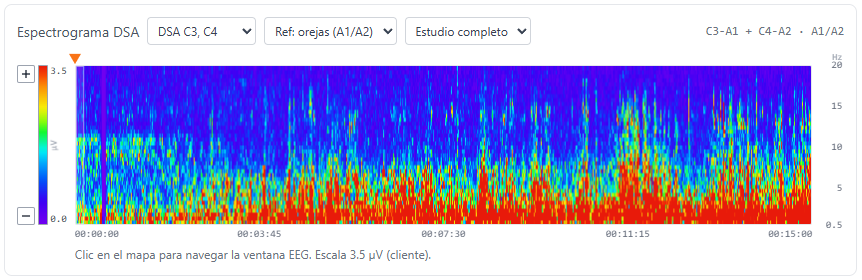
\includegraphics[width=\textwidth]{Chapter5/chapter5Figs/espectrograma_dsa.png}
    \caption{Visualización del espectrograma DSA
    implementado en EpilexIA.}
    \label{fig:espectrograma_dsa}
\end{figure}

\begin{nuevotexto}
La persistencia y la consulta de los resultados, el cálculo de los espectrogramas y las limitaciones de la implementación se detallan en el Anexo~B.
Las pruebas automatizadas de la API y del motor se resumen en la Sección~\ref{sec:pruebas-automatizadas}.
\end{nuevotexto}

\section{Despliegue e integración de los componentes}

El despliegue de EpilexIA comprende la configuración y puesta en
funcionamiento de los componentes que conforman el sistema, así
como el establecimiento de los mecanismos necesarios para su
comunicación y acceso a los recursos compartidos. La implementación
se organiza en proyectos independientes que incluyen la interfaz
web, el \textit{backend} clínico, la base de datos clínica, la API de
inteligencia artificial y el motor de procesamiento.

Para facilitar la construcción y ejecución de estos componentes,
se utilizan contenedores Docker y archivos de configuración
Docker Compose. Esta organización permite definir las dependencias
de ejecución, los puertos de comunicación, las variables de
entorno y los recursos de almacenamiento necesarios para cada
servicio.

La integración se realiza mediante una red Docker compartida,
servicios HTTP y mecanismos de persistencia. Asimismo, se
emplean volúmenes para conservar la información de las bases
de datos y permitir el acceso a los archivos electroencefalográficos
y a los modelos de clasificación.

\subsection{Entorno de despliegue en la nube}
\label{subsec:despliegue-nube}

EpilexIA se encuentra desplegado en infraestructura en la nube provista por la empresa BigQ, socio del sector privado del proyecto.
Sobre este entorno se realizaron las pruebas documentadas en el Capítulo~\ref{pruebas_evaluacion} y las sesiones de validación con la especialista del IPS, quien accede al sistema por internet desde el hospital.

El despliegue reúne en un servidor los componentes del sistema, ejecutados como contenedores mediante una configuración conjunta de Docker Compose.
Un servidor Nginx actúa como punto único de entrada: publica la aplicación web y encamina las solicitudes hacia el \textit{backend} clínico.
Las bases de datos, la API de inteligencia artificial y el motor de procesamiento no se exponen a internet y se comunican únicamente a través de una red interna.
Los archivos EEG y los modelos entrenados se almacenan en volúmenes compartidos entre los servicios que los requieren.

El acceso de los usuarios se realiza mediante HTTPS, bajo un dominio provisto por la empresa, cuya infraestructura incorpora además mecanismos de protección perimetral.
De este modo se atiende el requerimiento RNF-SEG-003.
La administración de estos elementos corresponde al proveedor de infraestructura y no forma parte del alcance de este trabajo.

Este entorno constituye la base operativa del sistema durante el proceso de transferencia al IPS, que prevé su despliegue en servidores propios de la institución.

\subsection{Contenedorización y configuración de servicios}

La contenedorización de los componentes de EpilexIA se implementa
mediante Docker, utilizando archivos \texttt{Dockerfile} para definir los
entornos de ejecución y configuraciones Docker Compose para
administrar los servicios asociados a cada proyecto. Esta
organización permite establecer las dependencias necesarias,
los comandos de inicio, las variables de entorno y los recursos
requeridos para el funcionamiento de las aplicaciones.

El Cuadro~\ref{tab:componentes-contenedorizados} resume los
principales componentes de ejecución de EpilexIA, indicando
las tecnologías utilizadas y las responsabilidades que
cumplen dentro del entorno contenedorizado.

\begin{table}[htbp]
    \centering
    \caption{Componentes contenedorizados del sistema EpilexIA.}
    \label{tab:componentes-contenedorizados}
    \small
    \begin{tabularx}{\textwidth}{|
        >{\raggedright\arraybackslash}p{0.27\textwidth}|
        >{\raggedright\arraybackslash}p{0.27\textwidth}|
        >{\raggedright\arraybackslash}X|}
        \hline
        \textbf{Componente} &
        \textbf{Entorno de ejecución} &
        \textbf{Responsabilidad principal} \\
        \hline

        \textit{Frontend} &
        Node.js (compilación) y Nginx (ejecución) &
        Compilación y publicación de la interfaz web. \\
        \hline

        \textit{backend} clínico &
        Java 21 y WildFly 39 &
        Ejecución de los servicios clínicos y las operaciones de negocio. \\
        \hline

        Base de datos clínica &
        PostgreSQL 17 &
        Almacenamiento persistente de la información clínica. \\
        \hline

        API de inteligencia artificial &
        Python, FastAPI y Uvicorn &
        Recepción de solicitudes y administración de ejecuciones y resultados. \\
        \hline

        Base de datos de inteligencia artificial &
        PostgreSQL 16 &
        Persistencia de ejecuciones, cola de trabajos y resultados del análisis. \\
        \hline

        Motor de inteligencia artificial &
        Python &
        Procesamiento de señales EEG y ejecución del modelo de clasificación. \\
        \hline
    \end{tabularx}
\end{table}

\subsection[Consideraciones operativas y limitaciones del despliegue]{Consideraciones operativas y limitaciones del \\despliegue}

En cuanto a las limitaciones del despliegue, el despliegue se encuentra distribuido entre
configuraciones Docker Compose individuales y una configuración conjunta utilizada en la nube.
No se dispone de un procedimiento único y completamente automatizado que abarque la preparación de todos los recursos, la inicialización de los servicios y la verificación integral de su funcionamiento.

Por otra parte, la utilización de una cola persistente
permite desacoplar la recepción de solicitudes de
inteligencia artificial de la ejecución de los trabajos.
Sin embargo, la disponibilidad del procesamiento
automatizado depende de que el motor se encuentre en
funcionamiento y pueda acceder tanto a la base de datos
de inteligencia artificial como a los archivos necesarios
para realizar el análisis.

Finalmente, no se evaluaron la escalabilidad, la tolerancia
a fallos ni el comportamiento del sistema bajo cargas elevadas.
La evaluación de estas propiedades requiere pruebas
específicas y condiciones de ejecución definidas,
que deben distinguirse de la descripción de los
mecanismos de contenedorización implementados.

\begin{nuevotexto}
La configuración de cada contenedor, las consideraciones operativas para la puesta en funcionamiento y la comunicación entre los componentes desplegados se detallan en el Anexo~B.
\end{nuevotexto}

